\section{Methods}

\subsection{Data}
%\subsubsection{Source}
The \texttt{PISCES Cull PDB} database server \citep{wang-2003} is a commonly used source for data for evaluating 
machine learning models trained to predict protein secondary structures.\\
In training our model, we have used the data set produced by \cite{zhou-and-troyanskaya-2014}, originally extracted from the PISCES server.\\
The data contains information on 5926 proteins. \citeauthor{zhou-and-troyanskaya-2014} have filtered the data such that it contains no proteins consisting of less than 50 or more than 700 amino acids, and have thus encoded each protein as a section of 700 amino acids, the non-existent ones (in the case of a protein of less than 700 amino acids) being marked as \texttt{Not Sequenced}.

\subsubsection{Features}
Each amino acid in the database contains 57 features (or channels) of information. The first 22 features encode which of the 20 amino acids that occur in genetic code, plus amino acid 'X' representing 'Unknown' as well as 'NoSeq'.\\
\\
This information is encoded in a one-hot format, meaning that instead of encoding the actual amino acid or the index of the acid, one encodes an array of zeros with only the element at the index of the number of the amino acid being set to one. So in order to encode Glutamic acid (E) i.e. the third\footnote{Interestingly, E is the third amino acid in the data set, even though it is the fourth amino acid if counting alphabetically. Refer to table 3 in the appendix for an alphabetically sorted list of amino acids.} amino acid, the one-hotted data would be $[0, 0, 1, 0, 0, ... , 0, 0]$. \\
Encoding the data in this way makes very good sense in regard to training classifiers, as if one was to encode amino acid E simply as the number 3 (E being the third amino acid), the classifier would falsely train on the premise that a guess of 4 was a less bad guess than a guess of 15, based on the proximity of the indices.\\
The secondary structure labels that the model attempts to predict are encoded in the same manner, however for training purposes we have collapsed them into indices in our model. Further, as explained above, there are three main forms of protein secondary structures (H, B, and C) and within them there are further 8 sub-forms of structures, as seen in  the Q8 table, which are the ones that are encoded in the dataset.

\end{multicols}
\begin{table}[h]
\centering
\begin{tabular}{l|l|l}
Feature nr.   & Feature                                     & Encoding                 \\ \hline
{[} 0,22{[}   & Amino acid residues                         & One-hot                  \\
{[}22,31{[}   & Secondary structure labels                  & One-hot                  \\
{[}31,33{[}   & N- and C-terminals                          & Binary                   \\
{[}33,35{[}   & Relative and absolute solvent accessibility & Binary                   \\
{[}35,57{[}   & Sequence profile                            & Probability distribution
\end{tabular}
\end{table}
\newpage
\begin{multicols}{2}
\noindent The binarily encoded N- and C-terminals indicate whether the amino acid in question is the first or the last in the protein chain.\\
While the solvent accessibility features in the PISCES database are encoded as floating point numbers, the creators of the dataset in question have followed the practice of \citeauthor{qi-et-al-2012} and discretizised the values to binary values. The threshold for absolute accessibility is 15, while relative accessibility is "is normalized by the largest accessibility value in a protein and thresholded at 0.15" \citep{zhou-and-troyanskaya-2014}.\\
The sequence profile in the final 22 features is calculated using the \textit{Position-Specific Scoring Matrix} (PSSM) system, and is used to indicate that if it had not been the amino acid in question that was present at this specific position, with what probability would it then statistically have been which of the other amino acids. Interestingly, the order of the amino acids in the sequence profile differs from that of the amino acid residues, however this should not have any impact on the model.


\subsubsection{Splitting the data}
When training our model, we split the above data into three sets: training, validation and test. The purpose of splitting the training data from the evaluation data is to counter possible overfitting, that is, training a model to an extent where it correctly predicts the kinks and quirks of the training set that do not express general tendencies in the system.\\
The point in further splitting into both a validation and a test set is that we continuously evaluate the loss and accuracy on the validation set (instead of the training set) in order to make decision regarding the architecture of the model and the configuration of the models hyperparameters. To prevent us from humanly overfitting to this set, the test set is held in reserve and is only evaluated once, in the end of a model's training (a so-called 'holdout dataset'), to evaluate how well the model does on new, never seen before data. After removing the test set the normal way of splitting the remaining data into training and validation set, is a split of 80\% to training, 20\% to validation \citep[p. 119]{goodfellow-et-al-2016}.\\
In this case though, we followed the advice from the documentation accompanying the dataset and split the data into 5430 proteins for training, 255 proteins for testing and 236 proteins for validation. The training set was then further shuffled between each epoch, to make sure that the batch gradient would be as close as possible to the true gradient, and reduce the risk of batches not being representative of the entire dataset.\\
In evaluating the optimal hyperparameters for the model we also iterated over different batch-sizes for training (results below).

\subsubsection{One-dimensional convolving}
When talking about convolutional neural networks, 2D-convolutions are usually what is meant, since the method is commonly used for image processing of one sort or another. In the case of image processing, a normal RGB image can be said to be comprised of three two-dimensional arrays of values, each representing one of the red, green or blue color channels.
\begin{Figure}
 \centering
 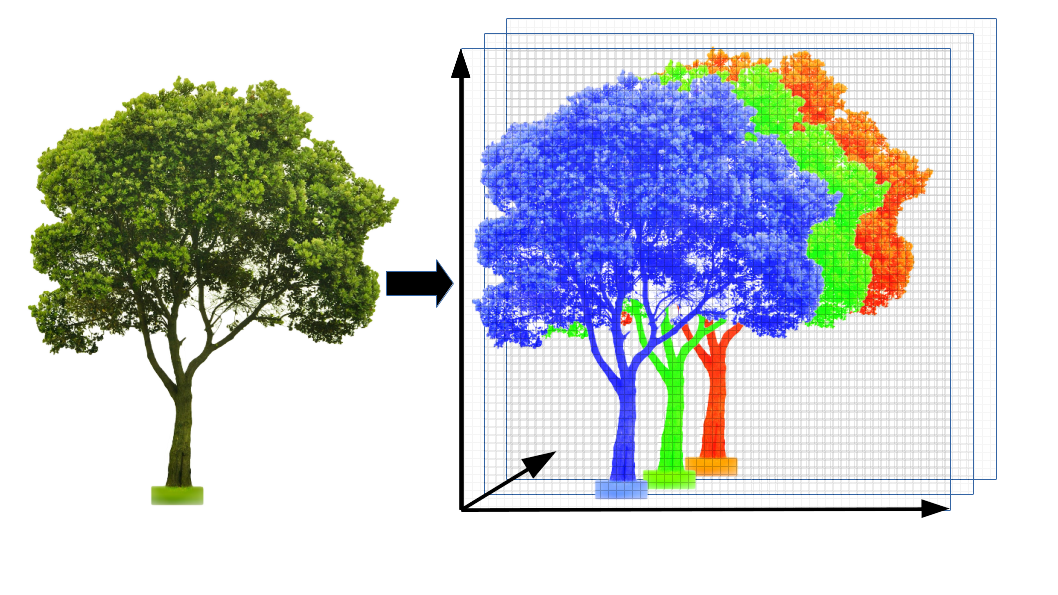
\includegraphics[width=\linewidth]{../graphs/tree/full}
 \captionsetup{width=0.8\linewidth, font=small}
 \captionof{figure}{An image of a tree, split into the three color channels.}
\end{Figure}
\noindent When convolving over such a picture using 2D-convolution, one can apply a series of two-dimensional filters, i.e. filters of a certain height and width.\\
This is however not the case with the CullPDB data. Our dataset is essentially one-dimensional, with a breadth of 700 amino acids, but instead of 3 color channels, it contains 57 features ("channels").
\begin{Figure}
 \centering
 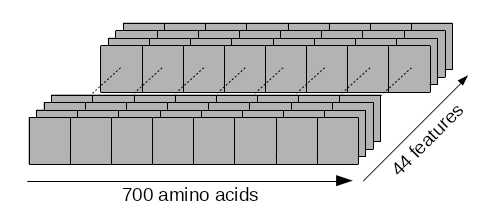
\includegraphics[width=\linewidth]{../graphs/tree/amino}
 \captionsetup{width=0.8\linewidth, font=small}
 \captionof{figure}{The input part of the dataset used in our models.}
\end{Figure}
\noindent Of these 57 features, we will be using the first 22 (amino acid residues) as well as the final 22 (the amino acid sequence profile) as input data, while in the end supplying an output of still 700 amino acids, but with 9 or 2 (secondary structures / solvent accessibility) channels for the single-task models and 11 (both) channels in the multi-task model.


\subsection{Tools}
\subsubsection{Model}
Being that we are training a convolutional neural network, in particular two sets of functions are important, namely activation and loss functions.

The activation functions we opted to use in this project were the rectifier, softmax and sigmoid functions respectively, whereas we use the Cross Entropy loss in evaluating and training the network.
\paragraph{Rectifier}
Possibly the simplest of these activation functions is the rectifier, which when implemented in an artificial neural network is referred to as a \textit{rectified linear unit} (ReLU). It is similar to linear units, with the difference that they do not allow negative values, but replace such values with zero.
\[
ReLU(x) = x^+ = max(0,x)
\]
\noindent Using ReLUs in artificial neural networks makes for easier optimization due to the fact that its derivatives remain large as well as consistent when the unit is active\citep[p. 189]{goodfellow-et-al-2016}.\\
As \citeauthor{goodfellow-et-al-2016} states: "Because rectified linear units are nearly linear, they preserve many of the properties that make linear models easy to optimize with gradient-
based methods. They also preserve many of the properties that make linear models generalize well."\citep[p. 170]{goodfellow-et-al-2016} Furthermore, they state that ReLU is the recommended activation function for most feedforward neural networks\citep[p. 170]{goodfellow-et-al-2016}.

\paragraph{Sigmoid function}
Sigmoid functions are a specific variant of logistic functions that serve to map values in arbitrary ranges to values within a specific range, so that the mapped values over the original values form a sigmoid curve. The value of applying sigmoid functions to outputs from a neural network is that they then enable the model to map its output of arbitrarily big or small values to a probability (i.e. a value $0\leq x \leq 1$). In the present case, this becomes relevant when predicting relative and absolute solvent accessibilities.
\[
Sigmoid(x) = \frac{1}{1 + e^{-x}} = \frac{e^x}{e^x +1}
\]

\begin{Figure}
 \centering
 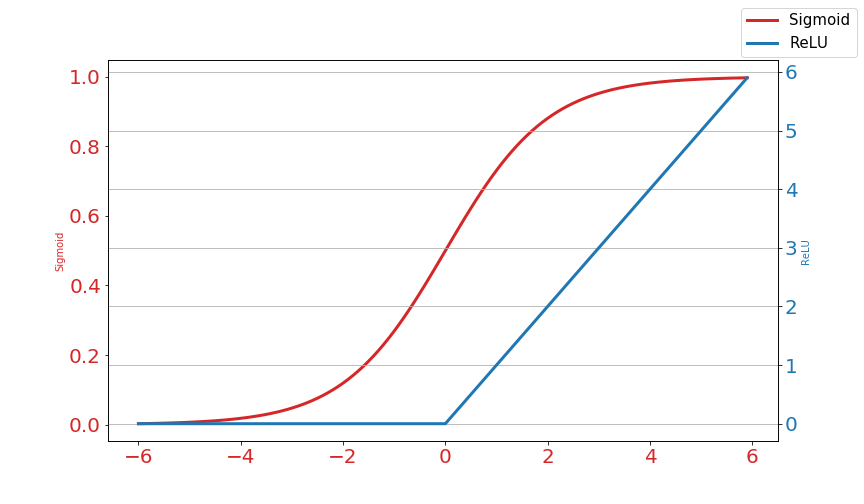
\includegraphics[width=\linewidth]{../graphs/activation.png}
 \captionsetup{width=0.8\linewidth, font=small}
 \captionof{figure}{The sigmoid and rectifier activation functions}
\end{Figure}

%\begin{wrapfigure}{I}{\linewidth}
%\centering
%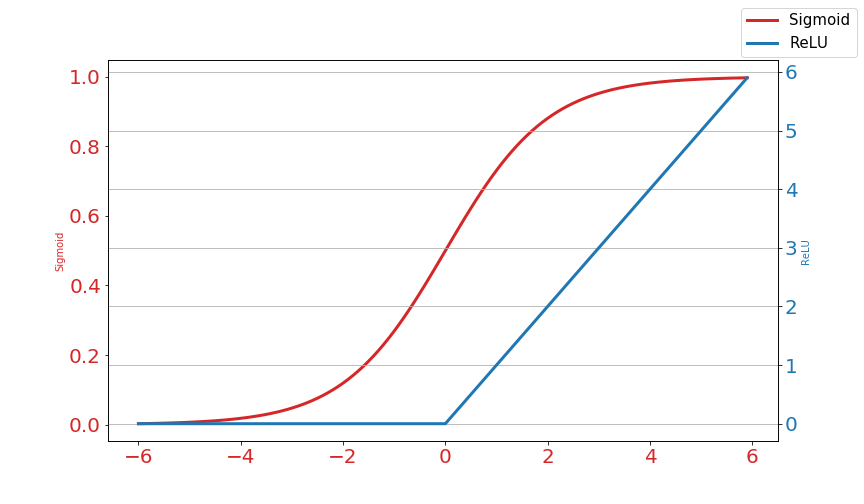
\includegraphics[width=\linewidth]{../graphs/activation.png}
%\caption{This is the former Share\LaTeX{} logo}
%\end{wrapfigure}

%\begin{figure}[h]
%  \centering
%  \frame{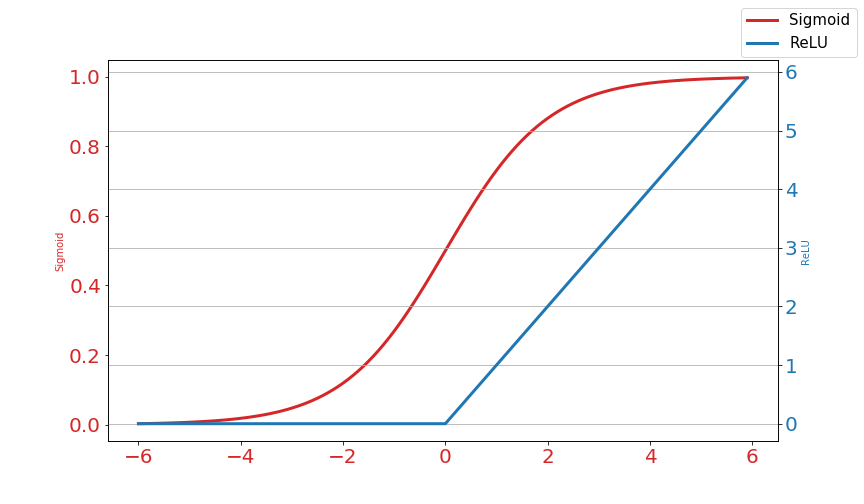
\includegraphics[width=\textwidth]{../graphs/activation}}
%  \caption{The sigmoid and rectifier activation functions}
%\end{figure}

\paragraph{Softmax}
The softmax function ($\sigma$) does very much the same as the sigmoid, only for a range of values. In other words, a set of non-normalized values (that is: of arbitrary length and spread) can via softmax be mapped to a probability distribution over that set. This means that all the values $x_i$ are in the range $0\leq x_i \leq 1$, and that they sum to 1.

This is especially relevant in cases where one is attempting to perform classification, such as which is the present case where we are training the model to predict amino acid secondary structures. 

Applying a softmax function on a dataset \textit{x} of \textit{j} elements would be as follows:
$$
\sigma(x_i) = \frac{e^{x_i}}{\sum_{j=1} e^{x_j}}
$$

\begin{Figure}
 \centering
 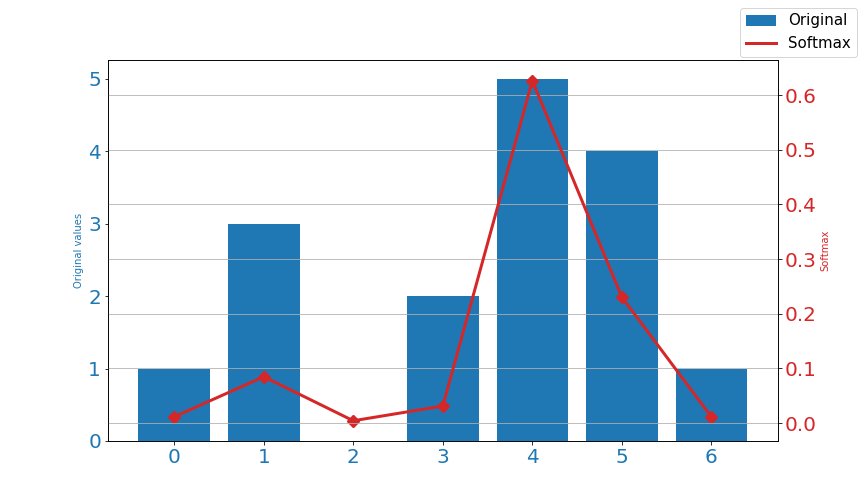
\includegraphics[width=\linewidth]{../graphs/softmax}
 \captionsetup{width=0.8\linewidth, font=small}
 \captionof{figure}{Example data softmaxed}
\end{Figure}
One will often see a very similar function called the \textit{Logarithmic Softmax} which resembles the above, but with the addition that the probability $\sigma(x_i)$ equals the natural logarithm of the same:
\[
\sigma_{log}\left(x_{i}\right)=\log \left(\frac{e^{ x_{i}}}{\sum_{j=1} e^{ x_{j}}}\right)
\]
In practical implementations this approach helps preventing possible underflows.

%\begin{figure}[h]
%  \centering
%  \frame{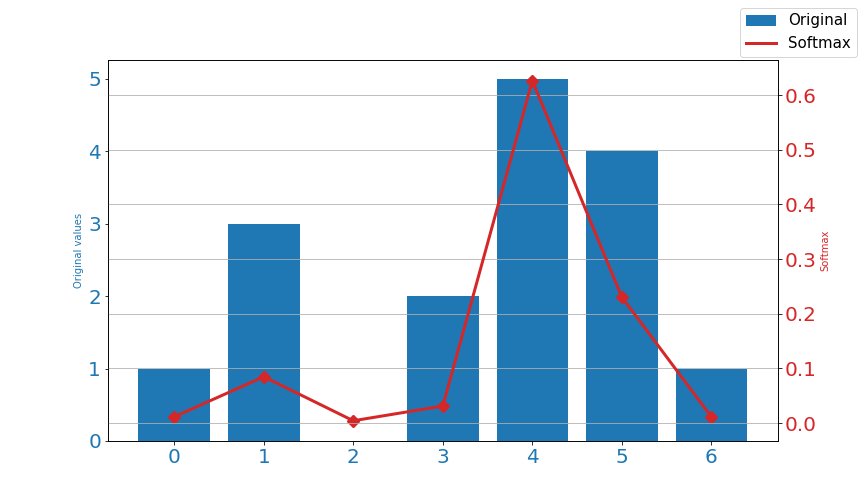
\includegraphics[width=\linewidth]{../graphs/softmax}}
%  \caption{Example data softmaxed}
%\end{figure}


\paragraph{Cross Entropy Loss}
Between two probability distributions each over the same set of outcomes there exists a certain cross entropy.
Thus, given two probability distributions \textit{m} and \textit{n} predicting the discrete outcome $\mathcal{Z}$, the formula for calculating the cross entropy is:
$$L ( m , n ) = - \sum _ { z \in \mathcal { Z } } m ( z ) \log n ( z )$$
A specific instance of the cross entropy loss is the \textit{binary cross entropy loss}, which is useful in cases where the possible outcome is binary (i.e. there are only two possible outcomes). 
\\
Seeing as the aim of this paper was to train our network to perform classifications first on amino acid secondary structures (of which there are eight) and then relative and absolute solvent accessibility (which are both encoded as either ones or zeros), we have used Cross Entropy Loss on the former and Binary Cross Entropy Loss on the two latter.


\paragraph{Optimization algorithm}
Several choices exist for the choice of optimization algorithm. One simple algorithm would be Stochastic gradient descent, in which there is one learning rate that applies to all model parameters (weights) and does not change throughout training.\\
Other optimizations such as Adaptive Gradient Algorithm (AdaGrad) maintains a learning rate for each parameter in the model, while algorithms such as the Root Mean Square Propagation (RMSProp) algorithm continuously adjusts the learning rate in accordance to the average magnitude in recent gradients.\\
In this project we have opted to use the Adam optimizer, introduced by \citeauthor{Adam} no more than four years ago. This optimizer combines two of the above aspects, namely individual learning rates for each parameter and continuous evaluation of the learning rates. However while RMSProp only evaluates the learning rate in response to the mean magnitude of gradients, Adam also evaluates on the variance of recent gradients.\\
To do this, \citeauthor{Adam} writes that the Adam optimizer has four configuration parameters: 
\begin{itemize}
\item $\alpha$: The initial learning rate,
\item $\beta_1$: The exponential decay rate for the mean of gradients
\item $\beta_2$: The exponential decay rate for the variance of gradients
\item $\epsilon$: A very small value useful to prevent division by zero
\end{itemize}
In the section 'Which optimizer to use?' of his 2016 article "An overview of gradient descent optimization algorithms" author \citeauthor{Ruder16} writes:

"Insofar, RMSprop, Adadelta, and Adam are very similar algorithms that do well in similar circumstances. \citeauthor{Adam} show its bias-correction helps Adam slightly outperform RMSprop towards the end of optimization as gradients become sparser. Insofar, Adam might be the best overall choice."\\
In this project we have chosen to follow the advice of \citeauthor{Ruder16} and use the Adam optimization algorithm.

\subsubsection{Technological implementation details}
In training our network we utilized a machine learning framework for Python called \href{https://pytorch.org/}{PyTorch}, specifically optimized for building deep neural networks. \\
The PyTorch library is build upon the \href{http://torch.ch/}{Torch} library, originally a machine learning library and language based on the scripting language Lua.\\
The strength in using PyTorch stems from several aspects:
\paragraph{GPU support}
PyTorch provides a strong framework for performing calculations on a graphical processing unit rather than the computer's CPU. While GPUs are valued in video game circles, they are also useful for performing machine learning tasks, since these are often tasks that involve a high number of calculations that can be performed in parallel. For this, a GPU is preferred over a CPU since they often have a much higher number of cores, and are thus better suited for parallel programming. Indeed in our case, there was a factor of 20 difference in the time needed to train an epoch between doing it on the CPU versus the GPU.
\paragraph{Tensors}
The main data structure used in the PyTorch framework is tensors. Where a vector is a 1-dimensional array and a matrix a 2-dimensional array, a tensor is a multi-dimensional array. This means they can be 1-, 2-, 3- or even 42-dimensional arrays. As such tensors subsume scalars, vectors and matrices \citep[p. 211]{goodfellow-et-al-2016}. Tensors in PyTorch are multi-dimensional arrays much like the ones implemented in numpy, but with the option to place them on the GPU rather than the CPU.
\paragraph{Automatic differentiation}
In order to utilize the backpropagation that lets neural networks train and improve, the loss must be differentiated in regards to all of the weights and values in the model in order to calculate the gradients. This can be a cumbersome task when performed by hand, but PyTorch provides a powerful tool for this in the \texttt{autograd} and \texttt{optim} modules. The first of these modules keeps track of which computations were performed on which variables in order to arrive at the final value of a variable, so that it can be retraced backwards in the end to calculate gradients, while the latter contains ready-made implementations of several optimization algorithms (among them Adam), which automatically adjusts the weights and values in the model according to the calculated gradient and a supplied learning rate.\\
These things combined allow a training step for a neural network to be performed in as few steps as shown below:
\begin{lstlisting}
# Setup
LR = 0.0025         # learning rate
optimizer = torch.optim.Adam(cnn.parameters(), lr=LR)
loss_func = nn.CrossEntropyLoss()

# One training step
output = cnn(x)
loss = loss_func(output, y)
optimizer.zero_grad()
loss.backward()
optimizer.step()
\end{lstlisting}

\paragraph{Ready-made implementations}
A final helpful aspect of using PyTorch for implementing artificial neural networks is the abundance of already implemented algorithms and functions. This adds the further detail to the implementation that several of the most often used functions have been written together for reasons of numerical stability. \\
For example, the aforementioned Cross Entropy Loss function, which when implemented in PyTorch also contains an implementation of the \texttt{LogSoftmax()} function. The documentation for PyTorch reveals that the implementation then becomes:

\begin{align*}
\operatorname{loss}(x, \text {class})&=-\log \left(\frac{e^{ x[\text {class}]}}{\sum_{j} e^{ x[j]}}\right)\\
&=-x[\text {class}]+\log \left(\sum_{j} e^{x[j]}\right)
\end{align*}

\noindent A similar circumstance is that of the Binary Cross Entropy loss, where PyTorch provides an implementation in the form of \texttt{BCEWithLogitsLoss()} which readily combines the Binary Cross Entropy Loss with a sigmoid function, again in order to provide numerical stability. In this case the implementation becomes: \\
\[
\ell(m, n)=L=\left\{l_{1}, \ldots, l_{N}\right\}^{\top}
\]
where
\[ \quad l_{n}=-w_{n}\left[n_{n} \cdot \log m_{n}+\left(1-n_{n}\right) \cdot \log \left(1-m_{n}\right)\right]
\]

\subsubsection{Hardware}
In terms of performing the calculations, all of our training of the model was done on a Dell PC with a 7th gen octocore Intel Core i7 CPU, 16GB of RAM and a Nvidia GeForce GTX 1050TI GPU with 4GB of RAM and 768 cores running Linux.

\subsection{Single-task secondary structure prediction}
We built a convolutional neural network, implemented using PyTorch in order to predict amino acid secondary structures from the amino acid residues as well as the sequence profile. We tested variations on number of layers, layer depth, kernel sizes and learning rate (results below) in order to maximize performance of the model. 

\subsubsection{Architecture}

The basic structure of the model remained unchanged throughout these test. The basics of the structure was comprised of following elements:
\begin{itemize}
\item It was to be a deep neural network (i.e. at least one hidden layer of neurons),
\item The layer depth was to remain the same throughout the network,
\item Sufficient padding was to be added to the convolving layers so that the breadth of the intermediary values remained the same (the 700 amino acids),
\item After each layer, save the last, the layer was activated using a rectified linear unit,
\item The model should not itself contain a SoftMaxing layer, since this was built into the loss function,
\item The model was evaluated and optimized based on the output of a Cross Entropy loss function,
\item The model was to be optimized based on the loss on the training set while being continuously humanly evaluated on the loss and accuracy on the validation set.
\end{itemize}

\begin{Figure}
 \centering
 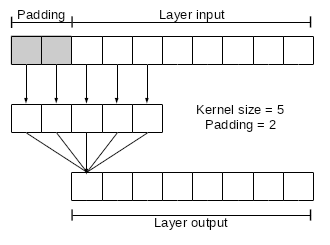
\includegraphics[width=\linewidth]{../graphs/padding}
 \captionsetup{width=0.8\linewidth, font=small}
 \captionof{figure}{The layer breadth is preserved across convolutions thanks to padding.}
\end{Figure}

\subsubsection{Accuracy}
Having built a network that was training and improving on the training set data, it was also relevant to evaluate the accuracy of the predictions of the network in addition to the calculation of loss on the validation set.\\
Several approaches to evaluating predictions exist. The output of our model was something of a proxy to a probability distribution, however not a true probability distribution since the model itself did not perform a SoftMax on the output. This was not an issue since the index of the largest value in a set of values remains the same before and after being SoftMaxed, and we could thus safely treat the index of the largest value in the un-SoftMaxed output as the label of the prediction.\\
In implementing a procedure to evaluate the accuracy of a prediction, we first collapse the output distribution as just described, and then produce a matrix of indicators as to whether the predicted label matched the label in the matrix of actual secondary structure labels as provided by the database.\\
Of course at this point the model would also be evaluated on its accurate prediction of padding (a task that proved remarkably manageable), and thus could achieve arbitrarily high accuracy just by adding more padding to the set. To avoid this, we construct a masking matrix from the values in the target set that are \texttt{NoSeq}. We then use this mask to filter out the irrelevant values in our matrix of correct and false predictions.\\
Finally taking the mean of this, now filtered, matrix of prediction correctness produces the percentage of the relevant predictions that were in fact correct.
\begin{Figure}
 \centering
 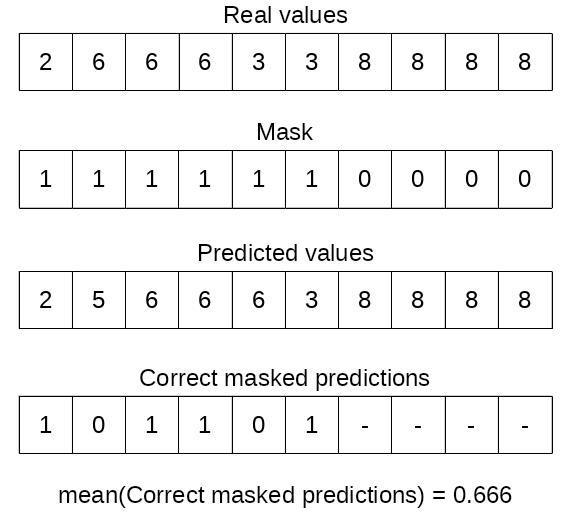
\includegraphics[width=0.8\linewidth]{../graphs/accuracy}
 \captionsetup{width=0.8\linewidth, font=small}
 \captionof{figure}{Calculating accuracy.}
\end{Figure}

\subsection{Single-task solvent accessibility prediction}
For comparison purposes, we also implemented a convolutional neural network to predict the two solvent accessibility features alone. This model is in most regards similar to the above, only with fewer output-channels and different final activation and loss functions.\\
One could think of the types of these three (structures, relative and absolute solvency) output as identical; the structure labels are a probability distribution while in a certain sense so are the solvent accessibility features - only a probability between two possible outcomes.\\
Nonetheless different final activation function were needed for the two latter, since performing a softmax on the binary output would always yield a 1. Thus the two solvent features are activated by a sigmoid function - effectively mapping their value to a probability between 0 and 1. Further, the loss function, now only distinguishing between two possible classes (0 and 1) should be the Binary Cross Entropy.\\
From a technical implementational perspective, as how in the previous model the SoftMax function was already included in the PyTorch implementation of BCELoss, in this case the sigmoid function is not explicitly stated in the model, as it is already included in the PyTorch module \texttt{BCEWithLogitsLoss} - the Binary Cross Entropy loss function.

\subsection{Multi-task learning}
%\subsubsection{Generelt om Multi-task learning}
There are multiple ways of implementing multi-task learning in artificial neural networks. The most basic distinction is between implementing the network using soft or hard parameter sharing. In the case of hard parameter sharing, the input data gets transformed through a number of layers in its entirety only then to be split into distinguishable output sets, and then optionally go through further set-specific layers. This approach provides a very strong line of defense against overfitting, as forcing the model to optimize on several predictive capabilities makes it less  susceptible to representing the aspects of the training data that are not representative of general tendencies in the domain. \\
In contrast to this stands soft parameter sharing, in which one could say that the model is comprised of a series of sub-models, each containing their own distinct layers and oriented towards each their prediction task. In this case the parameters of each of the models are balanced and regularized against each other in order to make them as similar as possible. \citep{ruder-2017}\\
On the grounds that the data set we are working with is somewhat limited (5926 proteins out of some 400.000 in the original PDB database) we were concerned about possible overfitting, and thus opted to implement our multi-task learning network with hard parameter sharing.

\subsubsection{Architecture}
Having decided on employing hard parameter sharing, we implemented the model in much a similar fashion to the single-task model explained above (i.e. convolutional layers, ReLU, padding, etc.). What sets the two models apart is the fact that in the final layer of the multi-task model the data is split up into the three output sets, secondary structure and relative/absolute solvent accessibility.\\
\\

\begin{Figure}
 \centering
 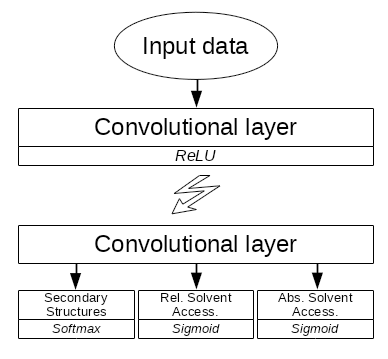
\includegraphics[width=\linewidth]{../graphs/arch}
 \captionsetup{width=0.8\linewidth, font=small}
 \captionof{figure}{Model architecture: The lightning represents one or more similar convolutional layers.}
\end{Figure}

\subsubsection{Training}
Utilizing the PyTorch loss function, autogradient and optimizer-libraries, implementing a model with essentially three losses is easy. As mentioned above, the model had a Cross Entropy loss for the secondary structure prediction, as well as two Binary Cross Entropy losses for the two solvency features. Training the model with regards to minimizing these losses is achieved simply by letting a variable be the sum of the three, and then letting the library automatically backtrace each of the parameters in the model via this value.
\begin{lstlisting}
# Calculate losses
loss1 = loss_func_structure(calc_struct,  correct_struct)
loss2 = loss_func_solvent(calc_rel, correct_rel)
loss3 = loss_func_solvent(calc_abs,  correct_abs)

# Sum the losses
loss_sum = (loss1 + loss2 + loss3)

# Backpropagate and train
loss_sum.backward()
optimizer.step()
\end{lstlisting}


\subsubsection{Accuracy}
Evaluating the accuracy of the model's predictions happens for each of the three features being predicted in the model.\\
The accuracy of the secondary structure label prediction happens in a similar fashion to the one in the single-task model. Seing as we know the structure of the solvent accessibility features to be binary and independent (an amino acid can be relatively solvent while not absolutely solvent and vice-versa), we can, after manually applying a sigmoid function on them, employ a simple round function to convert the probability outputted by the model to a binary prediction.\\
Having done so, the same method of constructing a matrix of correct and false predictions and then filtering this matrix by the mask already derived from the secondary structures was used.


\subsection{Hyperparameters}
In order to optimize our two models we iterated over a series of settings that helps control the learning algorithms behavior for the model. Those are the models' hyperparameters.
The hyperparameters of a model are not changed or learned by the model itself, but rather changed manually by us. As mentioned earlier, this is one of the purposes of a validation set. 
When finishing a training session on a model, we evaluate it against the validation set, and then change its hyperparameters to improve accuracy or counter overfitting. Not until satisfied with the parameters, and after training the final model, does one use the test set. \citep{goodfellow-et-al-2016} In our Convolutional Neural Network, the hyperparameters are: the number of layers, the depth of the layers, the learning rate and the size of the kernels used in the convolutions, as well as to a certain extend the batch size. The reason we have this reservation, is we could not freely change the batch size due to hardware limitations.\\
For a starting point, we chose to adapt the values used by \citeauthor{wang-et-al-2016}, and then iterated to both sides of those values.\\
An initial decision to make was the batch size - that is how many inputs from the data set to process at once. In general there are three approaches how many data points to train on at once, compared to the total length of the data (LOD):
\begin{center}
\begin{tabular}{l|c}
\hline 
Name & Size \\ 
\hline 
Batch gradient & Size = LOD \\ 

Minibatch gradient & 1 $<$ Size $<$ LOD \\ 

Generative Stochastic & 1 \\ 
\hline 
\end{tabular} 
\end{center}
In the case of Generative Stochastic networks, the model is continuously trained on random single data points, and is generally accepted to produce better predictions than both batch and mini-batch gradient descents, however at the cost of increased training time.\\
Batch gradient was not an option for us, for the simple practical reason that there was not enough memory on our GPU to handle the entire data set at once. We opted for a batch size of 4 throughout our tests in a compromise between predictive power and speed of training.\\
A test of accuracy over different batch sizes can be found in the appendix.\\
\\
When deciding on which hyperparameters to optimize and which not to, we decided to do tests and optimize the initial learning rate supplied to the Adam optimization algorithm, but not to try different values of the other three hyperparameters this algorithm takes. These are the $\beta_1, \beta_2$ and $\epsilon$ parameters, the first two of which control how quickly the learning rate falls as a product of the mean and variance of recent gradients, and the latter being a very small security measure to avoid divisions by zero. This decision was made on the grounds that in the original paper presenting the Adam algorithm, authors \citeauthor{Adam} declare that "Good default settings for the tested machine learning problems are: [...] $\beta_1 = 0.9$, $\beta_2 = 0.999$ and $\epsilon = 10^{-8}$" \citep[p. 2]{Adam}.\\
As these values are also the default values when instantiating an Adam optimizer object in PyTorch, they have not been specified in the code.









